\section{Method}\label{sec:method}

\subsection{Stimuli}\label{sec:stimuli}

All stimuli are photographs or renderings of real Ukrainian objects and documents that a Ukrainian reader would recognise. Only the photographic conditions are manipulated synthetically (framing and image quality, below), and a single word is edited in the near-word probe (Section~\ref{sec:probe}). The benchmark has three genres, each with its own independent source of ground truth.

\paragraph{Signage.} \NSign{} photographs of real signs in Ukrainian towns and villages were selected from Wikimedia Commons under free licences. They comprise street-name plates, shop and pharmacy fronts, notices (opening hours, quarantine and prohibition notices, nature-reserve rules), public-transport stops with timetables, memorial plaques and plaques of public institutions (schools, hospitals, libraries, a post office, police, an employment centre). The first author transcribed every image line by line at full resolution, zooming in on small print. Text that could not be confirmed (tiny print, damaged or partly hidden letters, small logos) was recorded separately as \emph{uncertain}. One photograph with a dense handwritten timetable was excluded. Quoting uncertain text counts as correct, but it is not required for coverage.

\paragraph{Packaging.} \NPack{} raw photographs of Ukrainian food packaging (ingredient panels and fronts) were taken from Open Food Facts, a collaborative database whose contributors photograph products in shops and at home. Next to each raw photograph, the database stores a Google Cloud Vision OCR result with a bounding box for every character, and this OCR is the ground truth. To make sure the OCR is reliable, an ingredient photograph is kept only if at least 60\% of the words in the contributor's independent transcription of the ingredients occur in the OCR. A front photograph is kept only if at least half of the words of the contributor's product name occur in it. The contributor's transcription, product name and brand are added as further accepted reference text.

\paragraph{Documents.} \NDocsCollected{} real documents were collected as PDF files with a text layer from official and public Ukrainian sources. They include application forms of the Pension Fund, the Ministry of Justice, the State Land Cadastre and city councils' administrative-service centres (ЦНАП); Ministry of Health medical forms (e.g., 086/о, 027/о, 106/о); patient leaflets of medicines; electricity and gas bills and tariff notices from regional suppliers and the energy regulator; bank application forms and consumer-credit passports; university and school documents; announcements of councils and the National Police; and pages of library bulletins with book annotations, the closest available text to the back cover of a book. For each document, a block of consecutive lines with up to 150 words was cut from the first page (from the richest of pages 2--4 for library bulletins, whose first page is a cover). It was rendered at 150~dpi, and the text layer, with word boxes split into character boxes, is the ground truth. The rendered page is then ``photographed'' as a sheet lying on a textured surface, with a random homography (small perspective distortion and rotation) and uneven lighting. As a quality gate, Tesseract must find at least 60\% of the text-layer words on the clean rendering. This rejected \NDocsRejected{} documents, e.g., bilingual forms and PDFs whose text layer did not match the visible glyphs. \NDoc{} documents remain.

\paragraph{Framing.} Packaging and document stimuli are assigned one of three framing conditions. \emph{Full frame} keeps the whole object. \emph{Crop} moves one frame edge (left, right or bottom) into the text area by 14--35\%, which cuts lines and words as happens when a blind user aims a phone imprecisely~\cite{gurari2018vizwiz}. \emph{Occlusion} places either a skin-coloured finger entering from the bottom edge or a specular glare highlight over a randomly chosen character. Because the position of every character is known, its visibility in the final frame can be computed. We test a $3\times3$ grid of points inside each character box. A character is \emph{visible} if at least 8 of the 9 points are inside the frame and not occluded, \emph{hidden} if at most 2 are, and \emph{partial} otherwise. For glare, a point counts as occluded where the highlight's opacity exceeds 0.85. A token is visible, hidden, or partial if its characters are mixed. Sign transcriptions have no character boxes, so signage photographs are used as photographed (full frame), with any cropping or occlusion they already contain.

\paragraph{Quality.} All stimuli are then scaled to 1024~pixels on the long side and assigned one of three quality levels. \emph{Clean} adds only mild sensor noise. \emph{Blur} applies a Gaussian blur with $\sigma\in[1.6,2.4]$~px and reduces contrast to 80--95\%. \emph{Severe} applies $\sigma\in[2.8,3.8]$~px, reduces contrast to 50--70\% and brightness to 65--90\%, and adds stronger noise. Images are stored as JPEG at the highest quality that keeps the file below 240~kB, because the model client silently drops larger image attachments. Within each genre, the (quality, framing) cells are balanced and assigned in a seeded random order.

\paragraph{Ground-truth categories.} Every ground-truth token is categorised as \emph{digits}, a \emph{common word} (present in a 290-thousand-word Ukrainian frequency list derived from OpenSubtitles\footnote{\url{https://github.com/hermitdave/FrequencyWords} (2018 release, CC BY-SA 4.0).}), or a \emph{name or rare word} (absent from it: brands, surnames, place names, technical terms). The benchmark contains \NImages{} images with \NGTTokens{} ground-truth tokens, of which \NGTNotVisible{} are not fully visible. Figure~\ref{fig:examples} shows examples.

\begin{figure}[t]
\centering
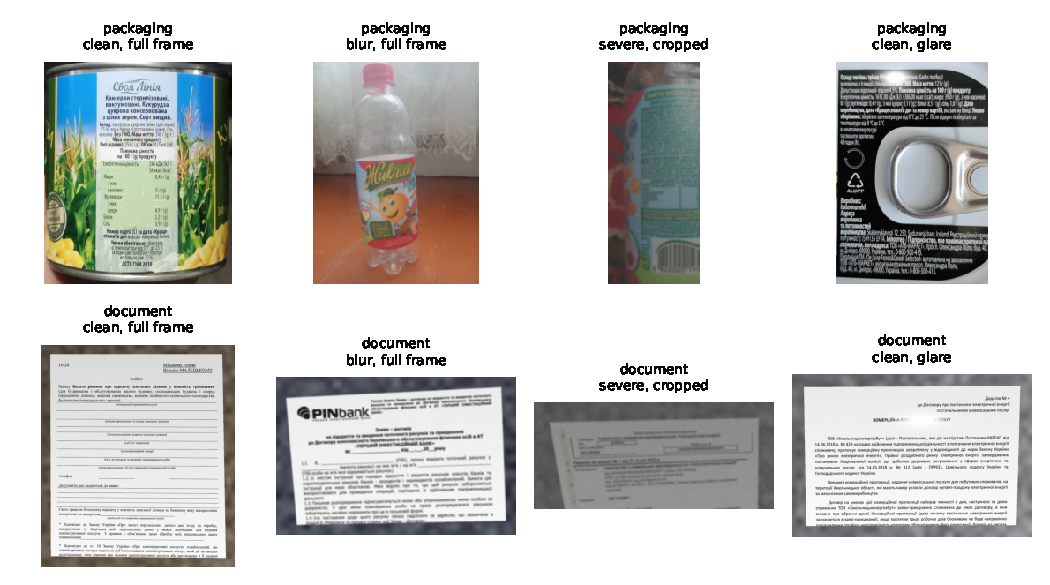
\includegraphics[width=\textwidth]{figures/fig_examples.pdf}
\caption{Example stimuli: real Ukrainian signage photographs (Wikimedia Commons), packaging photographs (Open Food Facts) and official documents, under different quality and framing conditions. For documents and packaging, the ground truth records every character and whether it is visible in the final frame.}\label{fig:examples}
\end{figure}

\subsection{Near-word probe}\label{sec:probe}

Prior-driven normalisation, where a model reports the word it expects rather than the word that is printed, cannot be measured on unedited text, because the printed and expected words coincide. We therefore edited the real document pages minimally. On each page, one common word of 6--12 letters that occurs once on the page was chosen at random. It was overpainted with a \emph{near-word}: the same word with one interior letter replaced by another letter of the same class (vowel or consonant), checked to be absent from the word list (e.g., \foreignlanguage{ukrainian}{«документ»}~$\to$~\foreignlanguage{ukrainian}{«докуцент»}, \foreignlanguage{ukrainian}{«сплатити»}~$\to$~\foreignlanguage{ukrainian}{«сзлатити»}). The near-word was typeset in a serif face at the original word's height and width, in the sampled ink colour. Each edited page was paired with its unedited original, and both were photographed with identical framing (full) and identical random degradation (clean or blur). Pages where the target word would be smaller than 11~px in the final image were skipped, leaving \NProbePairs{} pairs. In the description of each image we check whether the target is quoted in its printed form, whether the real word is quoted instead (normalisation), or whether some other form is quoted.

\subsection{Models and prompts}\label{sec:models}

We queried four production models from one vendor, spanning its capability and price range: Claude Haiku~5.5, Sonnet~5.5, Opus~5.5 and Fable~5.1, all on the \NImages{} benchmark images and the probe pairs. For cost reasons Fable~5.1, the most expensive model, received only the description prompt, and only descriptions were collected in the probe. All calls used the vendor's command-line client in non-interactive mode with default sampling settings, no tools and a short system prompt in Ukrainian: \foreignlanguage{ukrainian}{«Ти — сервіс опису зображень для незрячих і слабозорих користувачів. Відповідай українською мовою.»} (``You are an image-description service for blind and low-vision users. Answer in Ukrainian.''). Images were passed under opaque hashed file names so that the file name could not reveal the condition.

Two user prompts were used, each in a separate call without shared context. The \emph{description} prompt imitates a blind user's request: \foreignlanguage{ukrainian}{«Я незряча людина. Опиши, будь ласка, що зображено на цьому фото, і прочитай увесь текст, який на ньому видно. Увесь прочитаний текст наводь дослівно в лапках «…».»} (``I am a blind person. Please describe what is shown in this photo and read all the text that is visible on it. Give all the text you read verbatim in «…» quotation marks.''). The request for guillemets makes the claimed text machine-extractable without an additional model. The \emph{transcription} prompt asks for a verbatim line-by-line transcription, forbids corrections and completions, asks for a placeholder \foreignlanguage{ukrainian}{[нерозбірливо]} (``illegible'') where text is cut off, covered or unreadable, and asks for a ``(?)'' after any uncertain word. It serves both as a mitigation condition and as a run-time re-reading signal for detection.

\subsection{Extracting and labelling claimed text}\label{sec:labelling}

From each description we extract every guillemet-quoted span; an opening guillemet runs to the next closing one on the same line, so nested quotation marks cannot absorb descriptive prose. Straight and curly double quotes are also accepted. Bracketed or parenthesised remarks inside a quotation (e.g., \foreignlanguage{ukrainian}{«Осо[закрито пальцем] рахунок»}) are treated as annotations and removed, as are quotations that consist only of meta-words such as ``covered'' or of a single letter. Duplicate spans within a response are counted once. From each transcription, all lines are used after removing placeholders. Text is normalised by lower-casing, unifying apostrophe variants and mapping Latin look-alike letters inside Cyrillic words to Cyrillic. It is then split into letter and digit tokens. Digits separated by dots, colons or commas are merged, so dates, times and prices compare as units. Phone-like digit runs are also merged regardless of spacing, and leading zeros are dropped.

Each claimed token $o$ receives one label from the ground truth of its image, including the accepted reference text:
\begin{itemize}
\item \textbf{correct}: $o$ equals a visible token or a readable partial token, or $o$ is an explicit fragment (at least two characters) of a visible token or a contiguous run of the visible characters of a partial token;
\item \textbf{completion}: $o$ equals the full form of a token at least one of whose characters is hidden, i.e., the text is true but the camera did not capture it;
\item \textbf{misreading}: none of the above, but $o$ is within a normalised edit similarity of 0.5 of some ground-truth token, i.e., printed text was rendered wrongly;
\item \textbf{fabrication}: no ground-truth token is that similar, i.e., the text was invented.
\end{itemize}
A \emph{hallucinated} token is a misreading or a fabrication; \emph{unsupported} tokens additionally include completions. Misreadings are sub-typed as \emph{digit} errors, \emph{Ukrainian-letter} substitutions (the claimed and printed words differ only in \foreignlanguage{ukrainian}{і/и, ї/і, є/е, ґ/г} or contain letters that exist only in Russian), \emph{lexicalisations} (the claimed form is a real word or a known name but the printed one is not), and other substitutions. We also record whether the sentence containing a quotation carries a hedging cue (e.g., \foreignlanguage{ukrainian}{«ймовірно»}, \foreignlanguage{ukrainian}{«схоже»}, \foreignlanguage{ukrainian}{«нечітко»}, ``probably'', ``looks like'', ``blurry''). Matching against the image's token set rather than a forced alignment is deliberately conservative: a wrong number that happens to occur elsewhere on the same page counts as correct. Conversely, text that is printed but absent from the reference (e.g., a word the reference OCR missed) is counted as a fabrication, so the manual audit below is essential.

\paragraph{Audit.} To estimate the labeller's precision, the first author inspected a stratified random sample of \NAudit{} labelled tokens from all four models, with the quoted span and the printed line side by side, and judged whether each label was right.

\subsection{Detectors}\label{sec:detectors}

For each token quoted in a description, five signals are computed without access to the ground truth:
\begin{enumerate}
\item \emph{re-reading}: the token is absent from the same model's transcription of the same image; the variant \emph{re-reading uncertainty} fires when the transcription marks the token with ``(?)'';
\item \emph{cross-model}: the fraction of the other two main models whose description or transcription of the image does not contain the token;
\item \emph{OCR}: one minus the best normalised edit similarity between the token and any token Tesseract~5.5 (\texttt{tessdata\_best} Ukrainian model, page-segmentation modes 3 and 11 pooled) reads in the image~\cite{smith2007overview};
\item \emph{lexicon}: the token is not in the Ukrainian frequency list;
\item \emph{hedging}: the quoting sentence carries a hedging cue.
\end{enumerate}
Each signal is evaluated alone by the area under the ROC curve (AUROC)~\cite{hanley1982meaning}, and all signals are combined, together with the token's length and digit status, in a class-balanced logistic regression. Its scores are obtained by five-fold cross-validation with folds grouped by image, so that no image contributes to both training and testing. We report AUROC, average precision and, for deployment, the share of hallucinated tokens caught at fixed false-flag rates of 5, 10 and 20\% on correct tokens. We also evaluate a simple rule that needs no training: flag a token if the model's re-reading lacks it, or if neither OCR nor a majority of the other models confirms it.

\subsection{Statistics}\label{sec:stats}

Proportions are reported with Wilson 95\% score intervals~\cite{wilson1927probable}. Because tokens are clustered within images, we additionally report percentile intervals from a cluster bootstrap over images~\cite{efron1979bootstrap} (1000 resamples for rates and 300 for AUROC). Paired comparisons of the description and transcription prompts on the same images use the exact McNemar test on image-level outcomes. All analysis code and the response-free aggregate results are released (see Declarations). Raw model responses are withheld from the repository but can be regenerated with the released scripts.
